% Ejemplo de documento LaTeX
% Tipo de documento y tamaño de letra
\documentclass[12pt]{article}


\usepackage[spanish]{babel}
\usepackage{longtable} 
\selectlanguage{spanish}
\usepackage[utf8x]{inputenc}
\usepackage{graphicx}




% EL titulo, autor y fecha del documento
\title{Reporte de Actividad 3}
\author{Carlos Medina}
\date{20-2-15}


% Aqui comienza el cuerpo del documento
\begin{document}
% Construye el título
\maketitle


El siguiente reporte describirá los pasos realizados para la actividad 3 (2015-1), así como ilustrará los resultados de ésta.




\hspace {0.5cm} Fortran 90 (previamente FORTRAN) es un lenguaje de programación alto nivel de propósito general, procedimenta e imperativo, que está especialmente adaptado al cálculo numérico y a la computación científica. Es el sucesor de FORTRAN 77, informalmente conocido como Fortran 90 (y anterior a eso, Fortran 8X), fue finalmente lanzado como ISO/IEC estándar en 1991 y un ANSI estándar en 1992. En adición de cambiar el nombre oficial de FORTRAN a Fortran,además de agregar muchas características nuevas para reflejar los cambios significativos en la práctica de la programación que ha evolucionado desde el estándar de 1978.




\hspace {0.5cm} A continuación veremos unos cálculos que se resolverán utilizando Fortran 90, de calcular áreas a funciones.
\vspace {0.5cm}
     Primero empezaremos calculando el área de un círculoe en función del radio que tú elijas:
     
     \begin{verbatim}
     
     Program circle_area
  Implicit None
  Real *8 :: radius, circum, area
  Real *8 :: PI = 4.0 * atan(1.0)
  Integer :: model_n = 1
  print *, 'enter a radius:'
  read (*,*) radius
  circum = 2.0 * PI * radius
  area = radius * radius * PI 
  print *, 'Program number =' , model_n
  print *, 'radius =' , radius
  print *, 'circumference =' , circum
  print *, 'area =' , area
end Program circle_area 
 
    
     \end{verbatim}
     
Después de compilar, procedemos a ejecutar el programa y escrubir el radio que deseamos a nuesto gusto, entonces nos saldrá la siguiente pantalla:
   
     \vspace{2cm}

	\begin{center}
	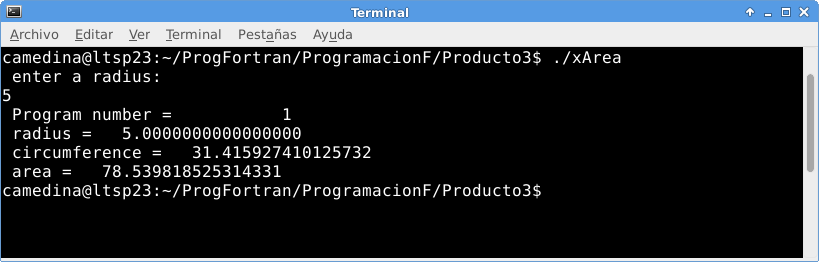
\includegraphics[width=13cm]{1.png}\\
	\end{center}
	
	\vspace{2cm}

Ahora probaremos con otro cálculo, por ejemplo, calcular el volumen de líquido en un tanque esférico de radio R, en el caso en que el nivel de líquido se encuentre a una altura H medida desde el fondo del tanque.Para esto, establecemos las variables y las formulas, después, tendremos este código:

\begin{verbatim}
   Program circle_area
  Implicit None
  Real *8 :: radius, high, diference, volume
  Real *8 :: PI = 4.0 * atan(1.0)
  Integer :: model_n = 1
  print *, 'Enter a radius:'
  print *, 'Enter high:'
  read (*,*) radius
  read (*,*) high
  diference = 3 * radius - high
  volume = 0.333 * PI * high * high * diference
  print *, 'Program number =' , model_n
  print *, 'radius =' , radius
  print *, 'High =' , high
  print *, 'Volume =' , volume
end Program circle_area 
\end{verbatim}

Se puede observar el uso de las variables reales como lo son el radio, la altura, para que te calcule el volumen. cabe recalcar que la variable "diference" fue agregada para facilitar el cálculo acorde con la fórmula.
Procedemos a compilarlo y cuando lo ejecutemos, saldrá el siguiente resultado:
\begin{center}
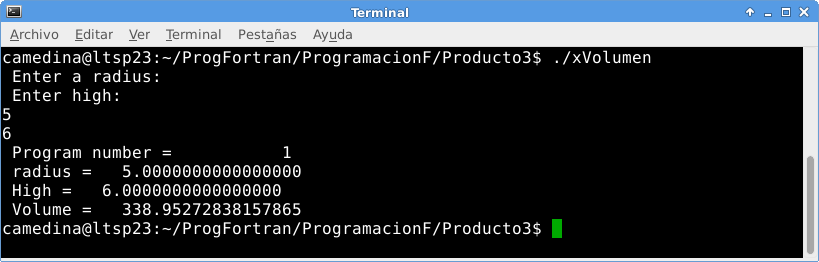
\includegraphics[width=13cm]{2.png}\\
\end{center}

Ahora, para el siguiente paso, se proporciona el siguiente código de doble precisión. Este codigo podrá a prueba los decimales que queramos para mejorar o simplificar la precisión.

\begin{verbatim}
	! Limits . f90 : Determines machine precision
! −−−−−−−−−−−−−−−−−−−−−−−−−−−−−
Program Limits
  Implicit None
  Integer :: i , n
  Real *8 :: epsilon_m , one
  n=60 ! Establish the number of iterations
  ! Set initial values :
  epsilon_m = 1.0
  one = 1.0
  ! Within a DO−LOOP, calculate each step and print .
  ! This loop will execute 60 times in a row as i is
  ! incremented from 1 to n ( since n = 60) :
  do i = 1, n , 1 ! Begin the do−loop
     epsilon_m = epsilon_m / 2.0 ! Reduce epsilon m
     one = 1.0 + epsilon_m ! Re−calculate one
     print * , i , one , epsilon_m ! Print values so far
  end do ! End loop when i>n
End Program Limits 
\end{verbatim}

Este código mostrará un valor que consta de muchísimas decimales, y con la precición asignada, $*8$, te muestra un total de 16 decimales, como se ve en la siguiente imagen.

\begin{center}
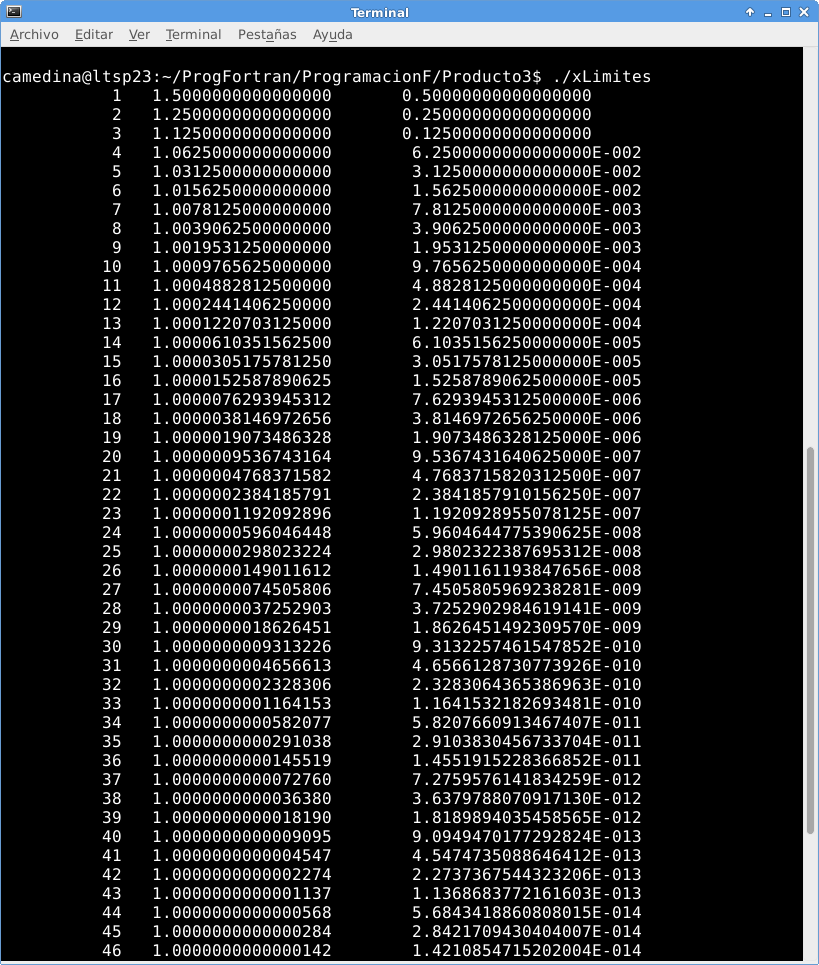
\includegraphics[width=13cm]{3.png}\\
\end{center}

Ahora, tratemos con cantidad menor de decimales, cambiando el valor $Real *8$ por $Real *4$ o símplemente $Real$ y así, nos dará 8 decimales solamente.

\begin{verbatim}
	! Limits . f90 : Determines machine precision
! −−−−−−−−−−−−−−−−−−−−−−−−−−−−−
Program Limits
  Implicit None
  Integer :: i , n
  Real *4 :: epsilon_m , one
  n=60 ! Establish the number of iterations
  ! Set initial values :
  epsilon_m = 1.0
  one = 1.0
  ! Within a DO−LOOP, calculate each step and print .
  ! This loop will execute 60 times in a row as i is
  ! incremented from 1 to n ( since n = 60) :
  do i = 1, n , 1 ! Begin the do−loop
     epsilon_m = epsilon_m / 2.0 ! Reduce epsilon m
     one = 1.0 + epsilon_m ! Re−calculate one
     print * , i , one , epsilon_m ! Print values so far
  end do ! End loop when i>n
End Program Limits 
\end{verbatim}

Compilamos, ejecutamos, y nos aparecerá:

\begin{center}
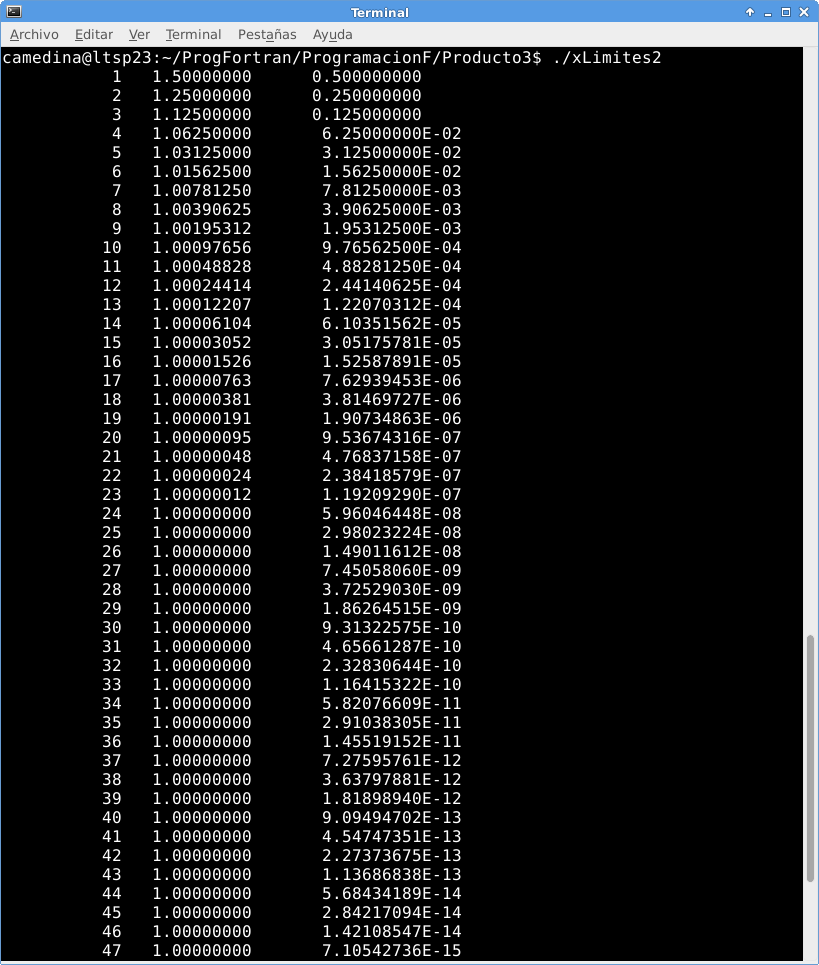
\includegraphics[width=13cm]{4.png}\\
\end{center}

Como podemos ver, cuando determinamos la presición, nos da el doble del número que elegimos ($*8$ para 16, $*4$ para 8).

	Fortran también maneja las funciones trigonométricas y las especiales. A continuación veremos un ejemplo de la función seno y la función exponencial.

\begin{verbatim}
!Math . f90 : demo some Fortran math functions
! −−−−−−−−−−−−−−−−−−−−−−−−−−−−−−−−−−−−−−−−−−
Program Math_test ! Begin main program
  Real *8 :: x = 1.0 , y, z ! Declare variables x, y, z
  y = sin (x) ! Call the sine function
  z = exp (x) + 1.0 ! Call the exponential function
  print * , x, y, z ! Print x, y, z
End Program Math_test ! End main program 
\end{verbatim}

Compilamos y nos saldrá el resultado.

\begin{center}
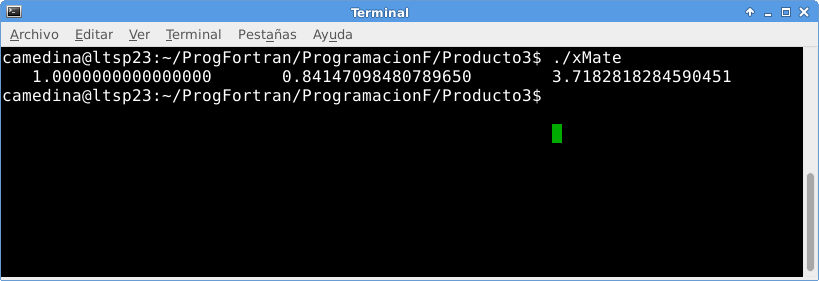
\includegraphics[width=13cm]{5.png}\\
\end{center}

Modificaremos el programa anterior para calcular la raíz cuadrada de -1; el arcoseno de 2.0; y el logaritmo de 0.

\begin{verbatim}
!Math . f90 : demo some Fortran math functions
! −−−−−−−−−−−−−−−−−−−−−−−−−−−−−−−−−−−−−−−−−−
Program Math_test ! Begin main program
  Real *8 :: x = -1.0 , y=2.0, z=0 ! Declare variables x, y, z, a, b, c
  a = sqrt (x) ! Call the sine function
  b = asin (y) ! Call the exponential function
  c = log (z)
  print * , x, y, z, a, b, c ! Print x, y, z
End Program Math_test ! End main program 
\end{verbatim}

Como se puede observar, se declaran las variables x, y, z (valores) y a, b, c (funciones), escribiendo después la orden para imprimir los resultados. Compilando y ejecutando se muestra lo dicho.

\begin{center}
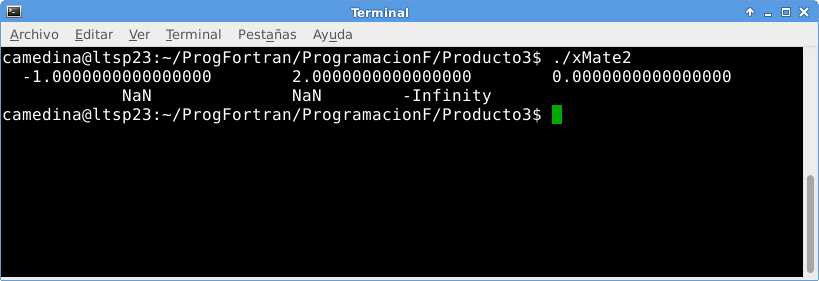
\includegraphics[width=13cm]{6.png}\\
\end{center}

También es posible calcular el valor de una función f(x, y) = 1 + sin(x y) definida por el usuario, escribiendo el siguiente código, compilándolo y ejecutándolo:

\begin{verbatim}
! Function . f90 : Program calls a simple function
! −−−−−−−−−−−−−−−−−−−−−−−−−−−−−−−
Real *8 Function f (x,y)
  Implicit None
  Real *8 :: x, y
  f = 1.0 + sin (x*y )
End Function f
Program Main
  Implicit None
  Real *8 :: Xin =0.25 , Yin =2. , c , f ! declarations ( also f)
  c = f ( Xin , Yin )
  write (*,*) 'f(Xin, Yin) = ' , c
End Program Main 
\end{verbatim}

\begin{center}
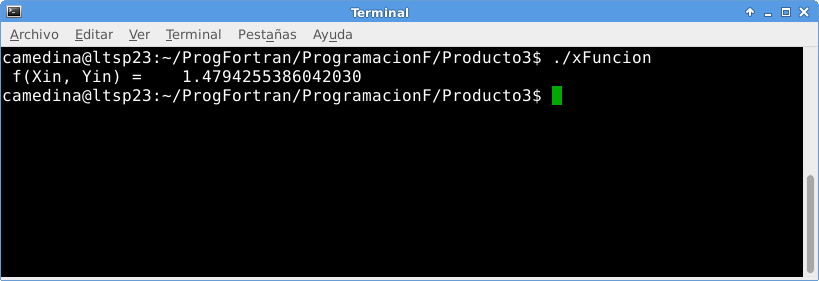
\includegraphics[width=13cm]{7.png}\\
\end{center}

Concluyendo con este reporte, es notable el hecho de que Fortran puede hacer bastantes calculos, y además de funciones, también se manejan subrutinas. Probaremos escribiendo el siguiente código:

\begin{verbatim}
! Subroutine . f90 : Demonstrates the call for a simple subroutine
! −−−−−−−−−−−−−−−−−−−−−−−−−−−−−−−−−−−−−−−−−−−−−
Subroutine g(x, y, ans1 , ans2 )
  Implicit None
  Real (8) :: x , y , ans1 , ans2 ! Declare variables
  ans1 = sin (x*y) + 1. ! Use sine intrinsic func.
  ans2 = ans1**2
End Subroutine g
Program Main_program ! Demos the CALL
  Implicit None
  Real *8 :: Xin =0.25 , Yin =2.0 , Gout1 , Gout2
  call g( Xin , Yin , Gout1 , Gout2 ) ! Call the subr g
  write (*,*) 'The answers are: ' , Gout1 , Gout2
End Program Main_program 
\end{verbatim}

Por último, compilamos y ejecutamos estos comandos.

\begin{center}
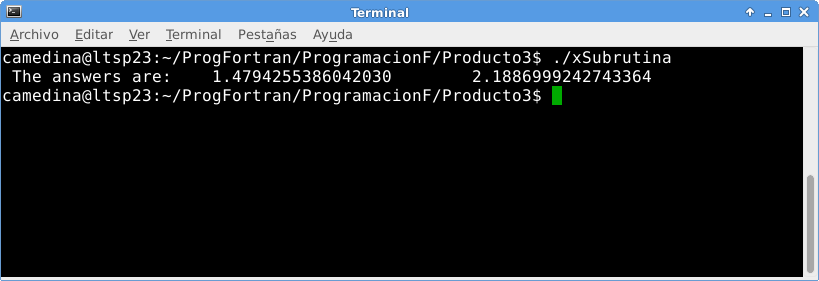
\includegraphics[width=13cm]{8.png}\\
\end{center}


% Nunca debe faltar esta última linea.
\end{document}
